% Template voor een kampprogramma van de
% Stichting Vierkant voor Wiskunde. Copyright 2000-2005,2011-2012:
% M.P. Alberts, J.C.C. Langeveld, M. Hendriks, W.J. Palenstijn.
% Meest recente update: 1-6-2012

% De 'begeleider' optie produceert een begeleidersversie.
% De 'deelnemer' optie produceert een deelnemersversie (zonder antwoorden).
% Zonder 'begeleider' en 'deelnemer' wordt een voorlopige versie gemaakt,
%  met antwoorden, en met de huidige datum aangegeven.

%\documentclass[begeleider]{kampprogramma}
%\documentclass[deelnemer]{kampprogramma}
\documentclass{kampprogramma}

\usepackage[utf8]{inputenc}
%\usepackage[dutch]{babel}
\usepackage{color}
\usepackage{hyperref}
\usepackage{url}
\usepackage{graphics}
\usepackage{gensymb}
\usepackage{wasysym}

\titel{Navigatie}

\auteurs{
Eveline Vissee\\
Gideon Wormeester\\
}

% ------- Hier de naam van het (.eps) bestand met de kaftillustratie
% Je kan dit commando ook weglaten als je nog geen plaatje hebt.
\illustratie{vierkantlogo}
% -------

% ------- Hier het kamp waarvoor het programma is. (A/B/C + jaar)
\kamp{Zomerkamp B 2018}
% -------


\begin{document}

\voorpagina

\voorwoord
\chapter*{Voorwoord}

In dit onderzoeksprogramma zoek je uit hoe mensen vroeger, voordat ze over smartphones met GPS beschikten, de weg vonden. We gaan het hebben over het bepalen van het Noorden (of Zuiden), breedte- en lengtegraden. We werken met het astrolabium om de tijd te bepalen aan de hand van de sterren.

Al in de Oudheid reisden handelaars de hele (bekende) wereld over met hun goederen; wat van ver komt is bijzonder en daardoor waardevol. Om op de juiste bestemming te komen is het niet praktisch om de weg uit je hoofd te leren, zeker niet als de reis maanden of jaren kan duren. De oudst gevonden kaarten komen dan ook uit de 25$^{e}$ eeuw voor het begin van onze jaartelling. 

Vroege schipskapiteins volgden vaak de kust om hun weg te vinden, maar dit was niet altijd genoeg. Om van Kreta naar Egypte te komen kostte meer dan een dag, waarbij het schip 's nachts niet in zicht van land was, en de bemanning dus de sterren moest gebruiken om het schip in de juiste richting te sturen. Zeekaarten werden gemaakt waarop ondieptes en opvallende kenmerken van de kust werden aangegeven.

Een andere vroege uitvinding was het peillood. Een zwaar gewicht dat achter het schip in het water gelaten werd kon gebruikt worden om de diepte van het water te bepalen, en daarmee kon de afstand tot het dichtstbijzijnde land worden geschat. Ook de wind kon helpen bij het bepalen van de richting.

De hemel was echter de meest nauwkeurige navigatiemethode op open zee. De Grieks-Egyptische geleerde Eratosthenes berekende in de tweede eeuw voor het begin van onze jaartelling de omtrek van de aarde door gebruik te maken van de stand van de zon. Zijn berekening was nauwkeuriger (en maar 10$\%$ groter dan de werkelijke waarde) dan die van Christoffel Columbus, meer dan 1500 jaar later.

's Nachts werd gebruik gemaakt van de sterren. De Poolster en de sterren van de Kleine Beer zijn heel geschikt om de richting van het Noorden te vinden, en het astrolabium, de sextant, octant en de jacobsstaf werden allen ontwikkeld om gebruik te maken van de sterren.




% ------- Legenda
%
% In de legenda worden symbolen voor opgaven uitgelegd.
% Alleen de daadwerkelijk in het programma gebruikte symbolen worden uitgelegd.
%
% De symbolen hebben de volgende betekenis:
% \ster : moeilijke opgave
% \vinger : deze opgave heeft een hint
% \schaar : dit is een praktische opdracht
% \gr : je mag/moet een grafische rekenmachine gebruiken voor deze opgave
% \discussie : dit is een discussie-opgave
%
% Zie het stukje 'Opgave' hieronder over hoe je de symbolen bij een opgave zet

\newpage
\legenda


\inhoudsopgave

% ------- Hier begint het eigenlijke programma

\section{Horloges}

We beginnen dit kampprogramma met een klein practicum. Gebruik hiervoor een horloge met wijzerplaat (misschien heb je er een bij je, misschien kun je je smartwatch instellen om een wijzerplaat te gebruiken). Anders kun je je begeleider vragen om het horlogewerkblad \textcolor{red}{MAAK HORLOGEWERKBLAD met lege wijzerplaat - iedere deelnemer heeft twee stuks nodig}.

Het doel van dit practicum is om het Noorden te bepalen. Als je je horloge gebruikt, zet het dan eerst gelijk met de wintertijd.

\begin{itemize}
\item Hoe laat is het nu?
\item Hoe laat is het nu -- in wintertijd? (hint: in maart gingen alle klokken een uur vooruit. In oktober gaan ze een uur terug. antwoord: dat betekent dat je nu een uur terug moet tellen.)
\end{itemize}

Als je het werkblad gebruikt, teken dan eerst de juiste stand van de wijzers op de wijzerplaat - in de wintertijd.

\textbf{LET OP:} kijk nooit rechtstreeks naar de zon! Ook niet als je een zonnebril draagt. Het is beter om te kijken naar de richting van de schaduwen.

\textcolor{red}{gebruik stok/parasol als zonnewijzer?}

Zorg dat de kleine wijzer van je horloge in de richting van de zon wijst. Op je werkblad, markeer de kleinste hoek tussen de kleine wijzer en de 12. Teken vervolgens de lijn die deze hoek precies in twee\"{e}n deelt.

\begin{itemize}
 \item Hoe wordt deze lijn ook wel genoemd? (antwoord: bissectrice)
 \item Deze lijn wijst precies naar het Zuiden. Teken nu op je werkblad de richting van het Noorden.
 \item Hoe weet je dat deze lijn precies naar het Zuiden wijst? (antwoord: om 12 uur, ofwel het middaguur, staat de Zon recht in het Zuiden. \textcolor{red}{aanvullen})
 \item Waarom werkt deze methode minder goed als je dichter bij de evenaar bent, en beter als je dichter bij de Noordpool bent? (antwoord: dicht bij de evenaar zijn de schaduwen korter en lijkt de zon altijd recht boven je te staan (en door de tilt van de aardas - $23.5^{\circ}$ werkt deze methode niet tussen de Kreeftskeerkring en de Steenbokskeerkring). 
 \item Hoe pas je deze methode aan voor de zomer? Zet je horloge terug op zomertijd en probeer of je dezelfde uitkomst krijgt. (antwoord: bepaal de kleinste hoek tussen de kleine wijzer en de 11.)
 \item Waarom werkt deze methode beter in de winter dan in de zomer? (antwoord: je hoeft geen rekening meer te houden met zomertijd, de zon staat lager dus je kan makkelijker de richting van de schaduwen bepalen, )
 \item De plaatselijke tijd hier in Nederland is hetzelfde als in het westelijkste puntje van Spanje (dat twee tijdzones verder naar het westen ligt), maar ook hetzelfde als in het oostelijkste puntje van Polen (dat twee tijdzones verder naar het oosten ligt). \textcolor{red}{KAARTJE VAN EUROPA MET TIJDZONES} Wat voor problemen levert dit op? Hoe pas je de methode aan?
 \item Hoe zou je deze methode aanpassen als je in Australi\"{e} was? (antwoord: richt de 12 van je horloge naar de zon, de bissectrice tussen de 12 en de kleine wijzer wijst nu naar het Noorden.)
\end{itemize}





\chapter{Je plaats op een ronde Aarde}

Wanneer je opzoekt waar je bent of waar je naar toe gaat, kijk je vrijwel altijd op een kaart. Of je dit nu doet met een papieren kaart, een informatiebord langs de weg of met een app op je telefoon, \'e\'en ding hebben ze gemeen: De kaart is plat. Maar de Aarde is allesbehalve plat en het vertalen van de ronde aarde naar een platte kaart is niet eenvoudig.

In dit hoofdstuk ga je leren wat er bij komt kijken om te navigeren op een ronde wereld en hoe het toch, met enige beperkingen, mogelijk is om platte kaarten te gebruiken voor een ronde Aarde.

\section{Co\"ordinaten op een boloppervlak}

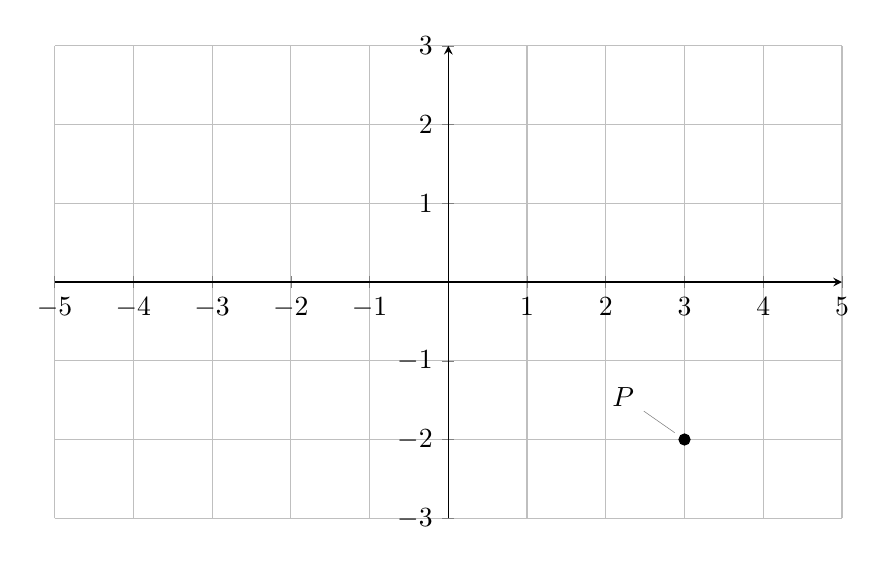
\begin{tikzpicture}
    \begin{axis}[axis lines = middle, grid = both, 
                 xmin = -5, xmax = 5, ymin = -3, ymax = 3,
                 x = 1cm, y = 1cm,
                 xtick = {-5, -4, -3, -2, -1, 0, 1, 2, 3, 4,5},
                 ytick = {-3, -2, -1, 0, 1, 2, 3}]
        \addplot[mark=*] coordinates {(3,-2)} node[pin=150:{$P$}]{} ;
    \end{axis}
	\label{fig_carthesisch}
\end{tikzpicture}

Hierboven zie je een voorbeeld van een plat rooster. Misschien heb je dit al eerder gezien tijdens de wiskundeles. Zo'n rooster zou je kunnen gebruiken om over een kaart heen te leggen. Langs de \textit{x}-as en \textit{y}-as staan getallen waarmee we de co\"ordinaten van punten in het rooster kunnen bepalen. Je kunt het punt met \textit{x} = 2 en \textit{y} = 3 vinden door op de \textit{x}-as de waarde 2 op te zoeken en op de \textit{y}-as de waarde 3. Het gezochte punt is vervolgens te vinden op de plek waar de 2 lijnen vanuit de gevonden punten op de assen elkaar snijden. Een korte notatie voor de co\"ordinaten van dit punt is $(2, 3)$.

\begin{opgave}
	\begin{subopgave}
		Waar ligt het punt (4, 1) in bovenstaand rooster?
		\begin{antwoord}		
			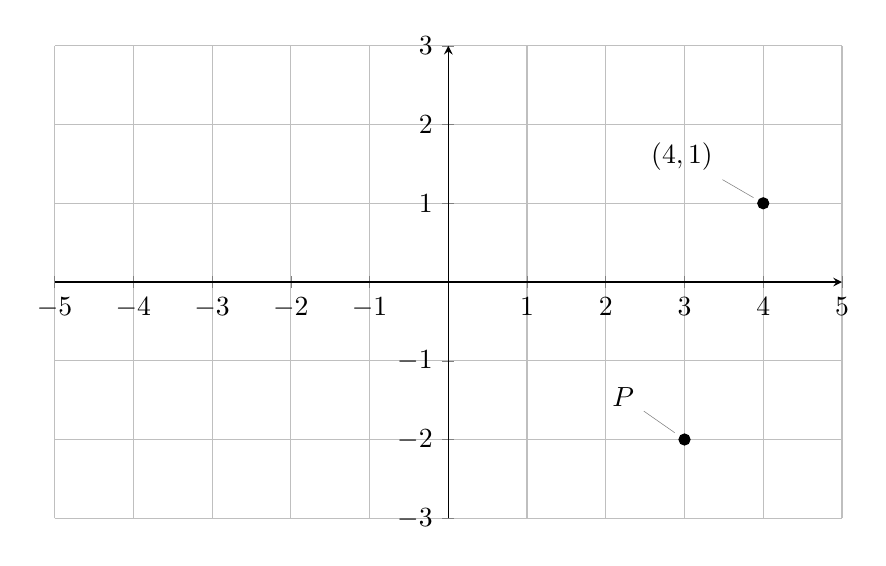
\begin{tikzpicture}
			    \begin{axis}[axis lines = middle, grid = both, 
		                 xmin = -5, xmax = 5, ymin = -3, ymax = 3,
                		 x = 1cm, y = 1cm,
        		         xtick = {-5, -4, -3, -2, -1, 0, 1, 2, 3, 4,5},
		                 ytick = {-3, -2, -1, 0, 1, 2, 3}]
			        \addplot[mark=*] coordinates {(3,-2)} node[pin=150:{$P$}]{} ;
			        \addplot[mark=*] coordinates {(4,1)} node[pin=150:{$(4, 1)$}]{} ;
			    \end{axis}
			\end{tikzpicture}
		\end{antwoord}
	\end{subopgave}
	\begin{subopgave}
		Wat zijn de co\"ordinaten van het in het bovenstaand rooster aangegeven punt P?
		\begin{antwoord}
			$(3, -2)$
		\end{antwoord}
	\end{subopgave}
\end{opgave}

Omdat de Aarde een bol is\footnote{Precies gezegd is de Aarde geen perfecte bol, maar een afgeplatte ellipso\"ide. De straal van de Aarde bij de evenaar is iets groter dan bij de polen. In dit onderzoeksprogramma gaan we echter uit van een bol.} hebben we voor plaatsen op het aardoppervlak een ander systeem van co\"ordinaten nodig, de zogenaamde bolco\"ordinaten. In plaats van \textit{x} en \textit{y} waardes, praten we over lengtegraden en breedtegraden.

\begin{figure}[h]
	\centering
	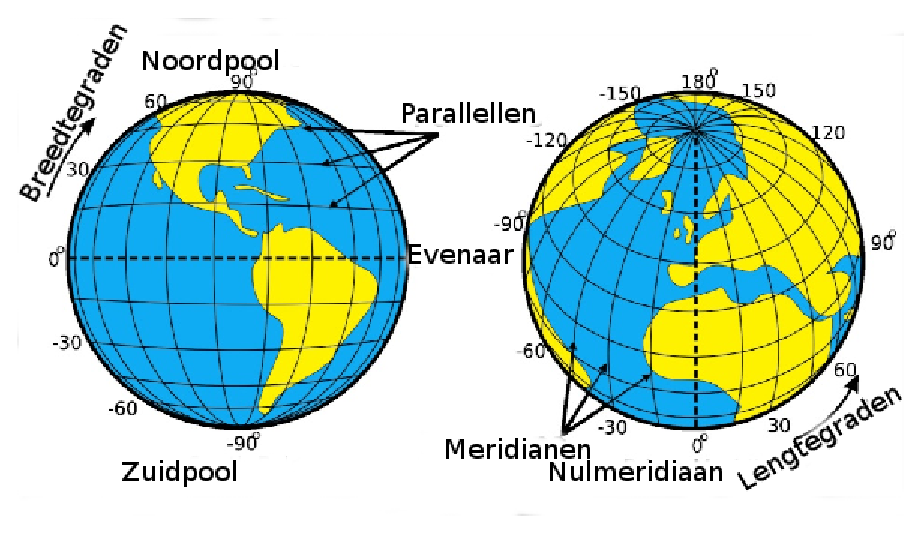
\includegraphics[width=15cm]{Parallels-and-Meridians-nl.eps}
	\caption{parallellen en meridianen}
	\label{fig_par_mer}
\end{figure}

De lengtegraad wordt gemeten langs de horizontale lijnen in bovenstaande figuur, terwijl de breedtegraad gemeten wordt langs de verticale lijnen. Lijnen met constante lengtegraad worden ook wel meridianen genoemd. Lijnen met constante breedtegraad heten parallellen. De belangrijkste meridiaan is de nul-meridiaan die door de Engelse plaats Greenwich loopt. Lengtegraden worden uitgedrukt ten opzichte van deze nul-meridiaan. Bij de parallellen is er een vergelijkbare situatie: De nul-parallel is beter bekend als de evenaar.

Lengte- en breedtegraden worden uitgedrukt in graden, zoals de naam al impliceert. Lengtegraden lopen van $-180\degree$ tot $+180\degree$ en breedtegraden van $-90\degree$ tot $+90\degree$. Meestal worden in plaats van min- en plus-tekens echter de windrichtingen gebruikt. Zo wordt een breedtegraad van $40\degree$ boven de evenaar geschreven als $40\degree N$ (N van Noord) en een lengtegraad van $15\degree$ ten oosten van de nul-meridiaan wordt geschreven als $15\degree E$ (E van East, oftewel Oost).

\begin{opgave}
	Lengtegraden hebben een totaal bereik van $360\degree$, terwijl breedtegraden slechts een bereik van $180\degree$ hebben. Waarom is het niet nodig dat breedtegraden ook een bereik van $360\degree$ hebben?
	\begin{antwoord}
		Neem een cirkel, deze stelt de $360\degree$ aan lengtegraden op de evenaar voor. Roteer de cirkel nu om een as die door het midden van deze cirkel loopt. Bij het roteren vormt zich een boloppervlak. Merk op dat de cirkel slechts $180\degree$ geroteerd hoeft te worden om een volledige bol te maken, niet $360\degree$. Als de breedtegraden ook een bereik van $360\degree$ zouden hebben, dan zou ieder punt op Aarde twee sets co\"ordinaten hebben.
	\end{antwoord}
\end{opgave}

\begin{opgave}
	\begin{subopgave}
		De straal van de Aarde is ongeveer 6400~km. Wat is de omtrek van de Aarde?
		\begin{antwoord}
			12800 km * $\pi$ = 40200 km
		\end{antwoord}			
	\end{subopgave}
	\begin{subopgave}
		Hoe ver moet je over de evenaar reizen om de lengtegraad van je positie met $1\degree$ te veranderen?
		\begin{antwoord}
			1/360 * 40200 km = 112 km
		\end{antwoord}
	\end{subopgave}
	\begin{subopgave}
		De parallel die door Heino loopt heeft een straal van ongeveer 3900~km. Hoe groot is de omtrek van deze parallel?
		\begin{antwoord}
			24500 km
		\end{antwoord}
	\end{subopgave}
	\begin{subopgave}
		Als je vanuit Heino $1\degree$ lengtegraad verplaatst, welke afstand leg je dan af?
		\begin{antwoord}
			$\frac{24500}{360} = 68$~km
		\end{antwoord}
	\end{subopgave}
\end{opgave}

Omdat het makkelijker is om het aardoppervlak plat weer te geven, hebben we een manier nodig om het bolvormige oppervlak op een plat rooster over te zetten. Een voor de hand liggende manier is om de boel zo af te beelden dat meridianen verticale lijnen worden op het platte rooster en parallellen horizontale lijnen.

\begin{figure}[h]
	\centering
	\includegraphics[width=15cm]{Equirectangular_projection_SW.eps}
	\caption{De aarde afgebeeld op een plat vlak}
	\label{fig_equirect}
\end{figure}

\begin{opgave}
	Op het aardoppervlak staan parallellen en meridianen loodrecht op elkaar. Blijft dat nog steeds zo als we het aardoppervlak op bovenstaande manier afbeelden?
	\begin{antwoord}
		Ja.
	\end{antwoord}
\end{opgave}

\begin{opgave}[\vinger]
	\begin{subopgave}
		In een plat rooster is de afstand tussen twee verticale lijnen overal hetzelfde. Is dit ook zo met meridianen op een boloppervlak?
		\begin{hint}
			Kijk nog eens naar je antwoorden 2 opgaven terug.
		\end{hint}
		\begin{antwoord}
			Nee, de afstand tussen meridianen neemt af naarmate je verder van de evenaar komt en wordt 0 bij de polen.
		\end{antwoord}
	\end{subopgave}
	\begin{subopgave}
		 Wat heeft dit voor gevolgen als we meridianen en parallellen als verticale en horizontale lijnen in een vlak rooster afbeelden?
		\begin{antwoord}
			Afstanden die gelijk zijn in de vlakke projectie zijn niet noodzakelijkerwijs gelijk op het boloppervlak. De projectie is dus niet afstand-behoudend.
		\end{antwoord}
	\end{subopgave}
\end{opgave}

Deze manier van het afbeelden van de Aarde op een vlakke kaart heeft dus duidelijke nadelen. Daarom gaan we later in dit hoofdstuk kijken naar verschillende manieren om de Aarde af te beelden. 

\section{De weg vinden met een kompas}
Lange tijd was het kompas een van de belangijkste navigatieinstrumenten en het wordt nog steeds regelmatig gebruikt. Een kompas is een eenvoudig apparaatje dat bestaat uit een metalen naald die vrij kan draaien, meestal boven een schijf waarvan richtingen kunnen worden afgelezen. Een kompas werkt onder invloed van het aardmagnetisch veld en de naald van het kompas zal altijd richting het noorden wijzen.

Richtingen op een kompas worden vaak aangegeven met de windrichtingen, bijvoorbeeld N (Noord), ZW (Zuidwest) of ZZW (Zuid-zuidwest). Naast windrichtingen is de richting ook uit te drukken in graden, van $0\degree$ tot $360\degree$. De richting van $0\degree$ komt overeen met N (en met $360\degree$).

\begin{opgave}
	\begin{subopgave}
		Welke windrichting komt overeen met $180\degree$?
		\begin{antwoord}
			Z (zuid)
		\end{antwoord}
	\end{subopgave}
	\begin{subopgave}
		Welke windrichting komt overeen met $225\degree$?
		\begin{antwoord}
			ZW (zuidwest)
		\end{antwoord}
	\end{subopgave}
	\begin{subopgave}
		Hoeveel graden horen er bij de windrichting ONO (oost-noordoost)?
		\begin{antwoord}
			$67.5\degree$
		\end{antwoord}
	\end{subopgave}
\end{opgave}

Een pad waarop constant dezelfde (kompas)koers wordt gevolgd wordt een "loxodroom" genoemd.

\begin{opgave}
	\begin{subopgave}
		Is er tussen twee punten op het aardoppervlak slechts \'e\'en loxodroom of  zijn er meerdere? Waarom?
		\begin{antwoord}
			Er zijn er meerdere. Merk op dat een loxodroom enkel vereist dat een constante kompaskoers gevolgd wordt, niet dat het het kortste pad is. In sommige vallen zijn er wel meerdere loxodromen die het kortste pad tussen twee punten vormen. Denk bijvoorbeeld aan de 2 polen. De meridianen zijn loxodromen.
		\end{antwoord}
	\end{subopgave}
	\begin{subopgave}
		Als je tussen twee punten reist en een zo kort mogelijke afstand wil afleggen, moet je dan een loxodroom volgen? Waarom wel/niet?
		\begin{antwoord}
			Nee. De kortste afstand tussen twee punten volgt een grootcirkel, wat meestal geen loxodroom is.
		\end{antwoord}
	\end{subopgave}
\end{opgave}

\begin{opgave}[\ster]
	\begin{subopgave}
		Bekijk de vlakke kaart van de Aarde in figuur~\ref{fig_equirect}. Is een rechte lijn op deze kaart altijd een loxodroom? In welke gevallen wel en in welke gevallen niet?
		\begin{antwoord}
			Nee. Alleen rechte lijnen die volledig verticaal of horizontaal lopen stellen loxodromen voor (met een koers van $0\degree, 90\degree, 180\degree, 270\degree$. 
		\end{antwoord}
	\end{subopgave}
	\begin{subopgave}
		Is de kaart uit de vorige sectie geschikt om kompaskoersen mee uit te zetten?
		\begin{antwoord}
			Nee. Omdat loxodromen niet per se rechte lijnen zijn op deze kaart, is het niet mogelijk om een directe kompaskoers te bepalen tussen twee punten. Als loxodromen wel rechte lijnen zouden zijn op de kaart, dan is het voldoende om simpelweg een rechte lijn tussen de twee punten te tekenen. Later komt een kaartprojectie aan bod waarbij dat mogelijk is. (Je kan hiervoor gedeeltelijk compenseren door gedurende korte tijd een bepaalde koers te volgen en dan je koers opnieuw te bepalen.)
		\end{antwoord}
	\end{subopgave}
\end{opgave}
	
Een kleine (of niet zo kleine, afhankelijk van waar je je bevindt) complicatie in het gebruik van een kompas is dat de magnetische noordpool van de Aarde niet hetzelfde is als de ware noordpool. Deze plaatsen liggen enige afstand uit elkaar. De as tussen magnetische noorden en magnetische zuiden is wat gekanteld ten opzichte van de rotatie-as van de Aarde, die door de ware noord- en zuidpool loopt.

Om deze reden zal een kompas dan ook vaak een afwijking hebben ten opzichte van het ware noorden.

\begin{opgave}
	\begin{subopgave}
		Waar denk je dat deze afwijking het grootst is?
		\begin{antwoord}
			Op de meridiaan die door de magnetische pool loopt, tussen de magnetische en ware pool. Als je hier richting de magnetische pool kijkt, dan bevindt de ware pool zich achter je.
		\end{antwoord}
	\end{subopgave}
	\begin{subopgave}
		Kun je plekken bedenken waar er juist geen afwijking is en het kompas ook naar het ware noorden wijst?
		\begin{antwoord}
			Op de meridiaan die door de magnetische pool loopt, behalve op het stuk tussen beide polen. Vanuit punten op deze meridiaan gezien liggen de magnetische en ware pool in elkaars verlengde.
		\end{antwoord}
	\end{subopgave}	
\end{opgave}

In werkelijkheid wordt de afwijking van een kompas niet alleen bepaald door het verschil tussen magnetische noorden en ware noorden, maar ook door allerlei magnetische eigenschappen van materialen die in de grond zitten. Moderne navigatie met behulp van een kompas maakt daarom gebruik van complexe kaarten waarop overal op Aarde de kompasafwijking wordt aangegeven. Deze afwijking verandert ook nog eens met de tijd, waardoor zo nu en dan nieuwe correctie-kaarten moeten worden gemaakt.

\section{Kaartprojecties}

Na dit intermezzo over het kompas, gaan we weer terug naar onze pogingen om het aardoppervlak op een kaart af te beelden.

Het afbeelden van de ronde Aarde op een plat vlak wordt ook wel een "kaartprojectie"  genoemd. Er zijn veel verschillende kaartprojecties met elk hun eigen voordelen en nadelen. In de vorige sectie ben je er al eentje tegengekomen. Deze projectie heeft vele namen, waaronder "vierkante platkaart"\ en "meridiaangetrouwe cilinderprojectie".

De term "meridiaangetrouw"  slaat op het feit dat met deze projectie lengtes van stukken die langs een meridiaan lopen (niet noodzakelijkerwijs dezelfde meridiaan) op schaal zijn. Dat wil zeggen dat twee stukken die elk een meridiaan volgen en op de kaart dezelfde lengte hebben, ook op de Aarde zelf dezelfde lengte hebben.

\begin{opgave}
	\begin{subopgave}
		Is deze kaartprojectie ook "parallelgetrouw"?
		\begin{antwoord}
			Nee. Dit is eerder aan bod gekomen in opgave 2.3 en 2.5.
		\end{antwoord}
	\end{subopgave}
	\begin{subopgave}
		Hoe zit het met afstanden van stukken die niet precies een meridiaan of een parallel volgen? Worden deze afstanden met constante schaal afgebeeld?
		\begin{antwoord}
			Nee.
		\end{antwoord}
	\end{subopgave}
\end{opgave}

Hoewel de vierkante platkaart een makkelijke projectie is om te maken en hij erg geschikt is om te werken met lengte- en breedtegraden van punten, heeft deze kaartprojectie een aantal belangrijke nadelen.

Een alternatieve kaartprojectie is de zogenaamde Mercator-projectie, genoemd naar de Belgische cartograaf Gerardus Mercator, die deze projectie als eerste heeft ge\"introduceerd. Hieronder staat een voorbeeld van de Mercator-projectie.

\begin{figure}[h]
	\centering
	\includegraphics[width=15cm]{Mercator_projection_SW.eps}
	\caption{Mercator-projectie}
	\label{fig_mercator}
\end{figure}
Een bijzondere eigenschap van de Mercator-projectie is dat deze richtingsgetrouw is. Dat betekent dat alle loxodromen rechte lijnen vormen op de kaart.

\begin{opgave}
	Als je als kapitein van een schip (zonder moderne hulpmiddelen) een route naar je bestemming moet vinden, gebruik je dan liever een vierkante platkaart of een Mercator-projectie? Waarom?
	\begin{antwoord}
		Een Mercator-projectie. Op deze kaart kan een koers worden bepaald door simpelweg het lijnstuk tussen oorsprong en bestemming te tekenen. Door tijdens de hele reis deze koers aan te houden, zal de bestemming uiteindelijk worden bereikt. Merk op dat deze koers niet per se de kortste route oplevert.
	\end{antwoord}
\end{opgave}

\begin{opgave}
	\begin{subopgave}
		Is de Mercator-projectie meridiaangetrouw?
		\begin{antwoord}
			Nee. De projectie strekt zich in principe tot in het oneindige uit richting de polen. Dat betekent dat een afstand langs een meridiaan dicht bij een pool op de projectie willekeurig lang kan worden.
		\end{antwoord}
	\end{subopgave}
	\begin{subopgave}
		Is de Mercator-projectie parallelgetrouw?
		\begin{antwoord}
			Nee. Om dezelfde reden als bij de vierkante platkaart: De kaart is overal even breed, terwijl de lengte van een parallel op het aardoppervlak niet overal gelijk is.
		\end{antwoord}
	\end{subopgave}
\end{opgave}

Hoewel de Mercator-projectie dus bepaalde voordelen biedt boven de vierkante platkaart, zijn er ook nadelen. Dit geldt voor alle projectie-methoden: Elke projectie heeft voordelen en nadelen. Omdat het aardoppervlak niet zonder vervorming is af te beelden op een platte kaart, moeten er altijd keuzes worden gemaakt. Afhankelijk van de gewenste eigenschappen kan de meest geschikte projectie worden gekozen.

\begin{opgave}
	Zoek op de Mercator-projectie Nederland op en zoek een ander punt op grote afstand van Nederland, maar wel op het noordelijk halfrond (bijvoorbeeld in Noord-Amerika of Azi\"e). Probeer de kortste afstand tussen deze twee punten op het aardoppervlak te tekenen.
	\begin{antwoord}
		Het antwoord is niet relevant. Verderop werken de deelnemers met een projectie die grootcirkels op rechte lijnen afbeeldt en kunnen ze de kortste afstand direct bepalen door een rechte lijn te trekken op die kaart. Dit kan dan vergeleken worden met hun eerste gok in deze opgave. Oplettende deelnemers zullen nu al opmerken dat het kortste pad geen rechte lijn is op de Mercator-projectie, omdat rechte lijnen loxodromen voorstellen en loxodromen in het algemeen niet samenvallen met grootcirkels.
	\end{antwoord}
\end{opgave}

Tot slot maken we kennis met de zogenaamde "gnomonische projectie". Dit is een bijzondere projectie waarin grootcirkels worden afgebeeld als rechte lijnen. Een grootcirkel is een cirkel over het aardoppervlak die het middelpunt van de Aarde als middelpunt heeft. Zo'n cirkel is de grootste mogelijke cirkel die over het aardoppervlak kan lopen.

\begin{opgave}
	Geef een voorbeeld van grootcirkel op het aardoppervlak.
	\begin{hint}
		Denk aan de parallellen. Welke parallel is het grootste?
	\end{hint}
	\begin{antwoord}
		De evenaar. Ook alle meridianen zijn grootcirkels.
	\end{antwoord}
\end{opgave}

Een belangrijke eigenschap van grootcirkels is dat het kortste pad tussen twee punten op een boloppervlak (in dit geval dus het aardoppervlak) altijd op een grootcirkel ligt.

\begin{opgave}
	De gnomonische projectie beeldt grootcirkels af op rechte lijnen. In welke situaties is dat handig?
	\begin{antwoord}
		De kortste route tussen twee punten is eenvoudig te bepalen met behulp van een gnomonische projectie.
	\end{antwoord}
\end{opgave}

Hieronder staat een voorbeeld van een kaart met gnomonische projectie. Merk op dat deze projectiemethode minder dan de helft van de Aarde in \'e\'en keer kan afbeelden en dat naarmate je dichter bij de rand komt, vervormingen steeds sterker worden.

\begin{figure}[h]
	\centering
	\includegraphics[width=10cm]{Gnomonic_projection_SW.eps}
	\caption{Gnomonische projectie}
	\label{fig_gnomonic}
\end{figure}

\begin{opgave}
	Zoek op de kaart met gnomonische projectie dezelfde twee punten op die je in opgave 2.13 ook al hebt opgezocht. Teken nu het kortste pad tussen deze twee punten en kijk terug naar wat je op de Mercator-projectie als kortste pad hebt aangegeven. Zat je dicht in de buurt met je eerste poging?
\end{opgave}

\newpage

\section{Astrolabium}

%\section{Avondpracticum}

\chapter{Moderne navigatie}

Hoewel navigatie met behulp van de sterren en instrumenten zoals een kompas en astrolabium eeuwenlang behoorlijk effectief was, kijken we in dit hoofdstuk naar een modernere vorm van plaatsbepaling en navigatie. Als je van een aantal punten exact de locatie weet, dan kun je dat gebruiken om zelf te bepalen waar je bent met behulp van een wiskundige techniek die "trilateratie" heet.

\section{Touwtjes-trilateratie}

\begin{opgave}
	Pak samen met iemand anders in jouw groepje een stuk touw en ga zo staan dat elk het touw bij het uiteinde vast heeft en het touw tussen jullie strak staat.

	Als je precies weet wat de positie is van de andere persoon en wat de lengte is van het touw, weet je dan ook precies wat jouw positie is? Waarom wel/niet?
	\begin{antwoord}
		Nee, als \'e\'en van de personen stil staat, kan de ander in een cirkel rondlopen.
	\end{antwoord}
\end{opgave}

\begin{opgave}
	Zoek nu een derde persoon uit jouw groepje en een tweede stuk touw. \'E\'en persoon houdt van beide touwen een van de uiteinden vast en de twee andere personen houden elk van \'e\'en van de touwen het andere uiteinde vast. Ga zo staan dat beide touwen strak staan.

	Als je precies weet wat de posities van de twee personen die \'e\'en touw vasthouden zijn en wat de lengte van beide touwen is, heb je dan voldoende informatie om de positie van de derde persoon te bepalen?
	\begin{antwoord}
		Alleen als de touwen exact in elkaars verlengde liggen. Als dat niet zo is, dan heeft het centrale punt de vrijheid om zich te bewegen in een cirkel rondom de rechte lijn tussen beide uiteinden. Als deze beweging zich tot twee dimensies beperkt, dan zijn er 2 punten waar de centrale persoon kan staan.
	\end{antwoord}
\end{opgave}

\begin{opgave}
	Herhaal het proces uit de vorige twee opgaven, maar nu met 3 stukken touw en 4 personen. \'E\'en persoon houdt van alle touwen \'e\'en uiteinde vast en de overige personen van elk touw ieder \'e\'en uiteinde.

	Kan de persoon met alle uiteindes in handen nu zijn of haar positie bepalen als de touwen allemaal strak staan en de posities 	van de overige personen en de lengtes van de touwen bekend zijn?
	\begin{antwoord}
		Als de touwen allemaal in hetzelfde vlak liggen, dat wil zeggen, als alle uiteindes op min of meer dezelfde hoogte worden 	vastgehouden, dan wel. Maar oplettende deelnemers merken wellicht op dat als de centrale persoon lager of hoger is dan de 			andere drie (bijvoorbeeld omdat deze bukt of op een meubelstuk staat), er nog een andere positie is waarin alle touwen 				strak staan.
	\end{antwoord}
\end{opgave}

Waar je in deze opgaven mee bezig bent geweest heet "trilateratie". Dit is een techniek om de positie van een onbekend punt te bepalen aan de hand van de posities van enkele andere punten en de afstand tot deze punten.

Trilateratie staat aan de basis van de techniek die vrijwel iedereen tegenwoordig gebruikt voor plaatsbepaling en navigatie: GPS. Voordat we verder gaan met GPS, kijken we eerst nog even verder naar trilateratie.

\section{Snijdende Cirkels}

\begin{opgave}
	We gaan met behulp van trilateratie de positie van een onbekend punt $P$ bepalen.
\begin{subopgave}
		Teken in je schrift een punt $A$. Als je weet dat het punt $P$ op een afstand van 3~cm van $A$ ligt, waar zou punt $P$ dan kunnen liggen? Teken de mogelijke locaties waar punt $P$ kan liggen in je schrift.
\end{subopgave}
\begin{subopgave}
		Teken een tweede punt $B$ op een paar centimeter van punt $A$. Als je weet dat het punt $P$ op een afstand van 4~cm van $B$ ligt, waar zou $P$ dan kunnen liggen? Teken de mogelijke locaties in je schrift. 
\end{subopgave}
\begin{subopgave}
		Hoeveel locaties zijn er die op de juiste afstand van zowel punt $A$ als punt $B$ liggen? Wat is er nodig om het punt $P$ op unieke wijze vast te leggen?
\end{subopgave}
\end{opgave}

In de vorige opgave heb je gezien dat in een plat vlak (zoals op een vel papier), je de positie van een punt vrijwel volledig kunt vastleggen als je de afstand tussen het punt en twee andere punten (met bekende positie) kent. De mogelijke posities zijn in dit geval de snijpunten van de cirkels rondom de punten waarvan de positie bekend is. In de meeste gevallen zullen dit twee snijpunten zijn.

\begin{opgave}
	Kun je een situatie bedenken waarin twee cirkels slechts \'e\'en punt gemeen hebben? Wat zegt dit over de plek van het onbekende punt ten opzichte van de bekende punten?
\end{opgave}

\begin{opgave}
	Tot hoeveel bekende punten moet je de afstand weten om zeker te zijn dat je de locatie van een onbekend punt op unieke wijze kunt bepalen als alle punten in een vlak liggen?
\end{opgave}

In een plat vlak is een cirkel de verzameling van punten die op een gegeven afstand van een centraal punt liggen.

\begin{opgave}
	Hoe ziet de verzameling punten die op een gegeven afstand van een centraal punt liggen er uit in drie-dimensionale ruimte?
\end{opgave}

Als je jouw afstand tot een vast punt kent, dan is jouw mogelijke locatie een punt op het boloppervlak om het bekende punt. Ken je de afstand tot 2 bekende punten, dan ligt jouw locatie op een snijpunt van twee boloppervlakken

\begin{opgave}
	Hoe ziet de verzameling van de snijpunten van twee boloppervlakken er uit?
\end{opgave}

Aannemend dat we niet in het grensgeval zitten waarbij de doorsnede van de twee boloppervlakken uit exact \'e\'en punt bestaat, hebben we dus nog niet voldoende informatie om de positie exact te bepalen.

\begin{opgave}[\vinger]
	Tot welke vorm krimpt de verzameling van snijpunten als we een derde vast punt met bekende afstand toevoegen?
	\begin{hint}
		De verzameling snijpunten van 2 boloppervlakken is een cirkel. Hoe ziet de verzameling snijpunten van een cirkel met een boloppervlak er uit?
	\end{hint}
\end{opgave}

\begin{opgave}
	\begin{subopgave}
		In drie-dimensionale ruimte, hoeveel bekende punten, waarvan je de afstand tot jouw locatie kent, zijn er nodig om altijd zeker te zijn dat je jouw locatie precies kunt bepalen? 
	\end{subopgave}
	\begin{subopgave}		
		In het gunstigste geval, wat is het kleinste aantal punten dat je nodig hebt voor plaatsbepaling?
	\end{subopgave}
\end{opgave}

Het Global Positioning System (GPS) werkt met dit principe van trilateratie. Een flink aantal satellieten draaien in diverse banen om de aarde. Deze satellieten zenden continu een signaal uit met, onder andere, hun huidige positie. Als een GPS ontvanger (bijvoorbeeld een smartphone) de positie van deze satellieten weet en kan meten wat de afstand is tussen de ontvanger en voldoende satellieten, dan kan de ontvanger z'n positie uitrekenen.

Als de ontvanger van onvoldoende satellieten een signaal ontvangt, dan is nauwkeurige plaatsbepaling niet goed mogelijk. Toch zijn er methodes om in dergelijke situaties met redelijke aannames de plaats te bepalen.

\begin{opgave}
	Als de ontvanger \'e\'en satelliet te weinig kan ontvangen, hoe zou deze dan alsnog z'n locatie kunnen bepalen?
	\begin{antwoord}
		Met \'e\'en satelliet te weinig zijn er 2 mogelijke locaties waar de ontvanger zich zou kunnen bevinden. Maar in vrijwel alle gevallen bevindt slechts 1 van de 2 mogelijke locaties zich op het aardoppervlak. Het andere punt kan uitgesloten worden omdat het zich diep onder de grond of hoog in de lucht bevindt.
	\end{antwoord}
\end{opgave}

\section{Plaatsbepaling zonder tijd?}

Hiervoor hebben we gezien hoe we onze locatie kunnen bepalen als we de afstand kennen tot 4 (of meer) satellieten, we onze exacte locatie kunnen bepalen. Maar het probleem is nu: Hoe bepaalt een GPS ontvanger de afstand tot een satelliet?

\begin{opgave}[\discussie]
	Bespreek met je groepje of je een manier kunt bedenken waarmee een GPS ontvanger de afstand tot een satelliet kan bepalen.
\end{opgave}

Het signaal van een satelliet verplaatst zich met de snelheid van het licht, ongeveer 300.000 km/s. Dus als de GPS ontvanger kan meten hoe lang het signaal onderweg is geweest van de satelliet naar de ontvanger, dan kan daarmee de afstand worden berekend.

\begin{opgave}
	Bedenk een manier waarop de ontvanger kan bepalen hoe lang het signaal onderweg is geweest.
	\begin{antwoord}
		Er zijn meerdere mogelijkheden. Een mogelijkheid is dat de satelliet op vooraf vastgestelde tijdstippen een signaal verstuurt (bijvoorbeeld iedere seconde). Een andere mogelijkheid is dat het tijdstip van verzenden als boodschap met het signaal mee wordt gestuurd. In alle gevallen is het essentieel dat de GPS ontvanger een nauwkeurige klok heeft.
	\end{antwoord}
\end{opgave}

GPS satellieten hebben zeer nauwkeurige atoomklokken aan boord. In het signaal van een GPS satelliet zit het tijdstip van verzenden verwerkt. Door het tijdstip van verzenden te vergelijken met het tijdstip van ontvangst kan de ontvanger bepalen hoe lang het signaal onderweg is geweest.

\begin{opgave}
	\begin{subopgave}
		Als de klok van de GPS ontvanger 0,1 seconde afwijkt van de klok van de GPS satelliet, hoe groot is dan de afwijking in de afstand die de ontvanger uitrekent?
	\end{subopgave}
	\begin{subopgave}
		Wat als de afwijking van de klok 0,01 seconde is? Of 0,001 seconde?
	\end{subopgave}
	\begin{subopgave}
		Veel GPS ontvangers kunnen de plaats op enkele meters nauwkeurig bepalen. Maak een schatting van hoeveel een klok maximaal mag afwijken van de satellietklok om een dergelijke nauwkeurigheid te behalen. Is dit realistisch?
	\end{subopgave}
\end{opgave}

In plaats van het inbouwen van een zeer nauwkeurige klok in iedere GPS ontvanger, is het veel makkelijker om bij elke plaatsbepaling de tijd uit te rekenen aan de hand van de signalen van satellieten.

\begin{opgave}[\ster\vinger]
	Als de ontvanger geen (nauwkeurige) klok bevat, wat is er nodig voor de ontvanger om met behulp van de satelliet signalen de tijd bepalen?
	\begin{hint}
		Bedenk dat de ontvanger nu naast de co\"ordinaten $(x, y, z)$ ook de tijd $t$ moet bepalen. Beschouw je tijd als een extra dimensie, dan moeten er dus eigenlijk de co\"ordinaten $(x, y, z, t)$ bepaald worden.
	\end{hint}
	\begin{antwoord}
		In plaats van de co\"ordinaten in drie-dimensionale ruimte, moeten de co\"ordinaten in vier-dimensionale ruimte-tijd worden bepaald. Net zoals de overstap van 2 naar 3 dimensies betekent dat het minimale aantal bekende punten stijgt van 3 naar 4, zorgt de stap van 3 naar 4 dimensies ervoor dat het minimale aantal punten stijgt naar 5. Er zijn dus 5 satellieten nodig voor een nauwkeurige plaatsbepaling als de ontvanger geen nauwkeurige klok heeft (zonder gebruik te maken van extra aannames zoals dat de ontvanger zich dicht bij het aardoppervlak bevindt).
	\end{antwoord} 
\end{opgave}

\section{De navigatie vergelijkingen}

De vergelijkingen voor plaatsbepaling en een aanpak om deze op te lossen. Ik weet nog niet of dit niet te moeilijk / lang is voor de doelgroep. 

% ------- Hier eindigt het eigenlijke programma

\hintsantwoorden

\end{document}
